% Un articolo scritto con LaTeX
\documentclass[a4paper]{book}
\usepackage[T1]{fontenc} % codifica dei font
\usepackage[utf8]{inputenc} % lettere accentate da tastiera
\usepackage[english,italian]{babel} % lingua del documento, quella finale è la principale
\usepackage[onlyinclude]{frontespizio}
\usepackage{tabularx}
\usepackage{ltablex}
\usepackage{booktabs}
\usepackage{multirow}
\usepackage{graphicx}
%\usepackage{afterpage}

\begin{document}
	\includefront{frontespizio-frn.pdf}
	
	\chapter{Descrizione del progetto}
	\section{Descrizione e requisiti}
	
	Si chiede la progettazione di una base di dati per tracciare le occasioni di contatto tra persone per recuperare informazioni sulla possibile diffusione del virus. Degli utenti va memorizziato: la possibile relazione (parentela, essere colleghi di lavoro); I luoghi in cui sono stati presenti; occasioni di contatto; tamponi e stato sierologico; informazioni sulla eventuale malattia. Si possono integrare in modo autonomo le specifiche.
	
	\chapter{Progettazione concettuale}

	
	In questo capitolo inizia la progettazione della base di dati al livello di astrazione più alto.
Dal risultato dell’analisi dei requisiti che devono essere soddisfatti si arriverà ad uno schema
concettuale indipendente dalla struttura dei dati e dall’implementazione fisica. In tale schema
concettuale, che verrà rappresentato usando un class diagram UML, si evidenzieranno le entità
(concetti) rilevanti ai fini della rappresentazione dei dati e le relazioni che intercorrono tra esse.
Si delineeranno anche eventuali vincoli da imporre.
	
	\section{Class diagram}
	
       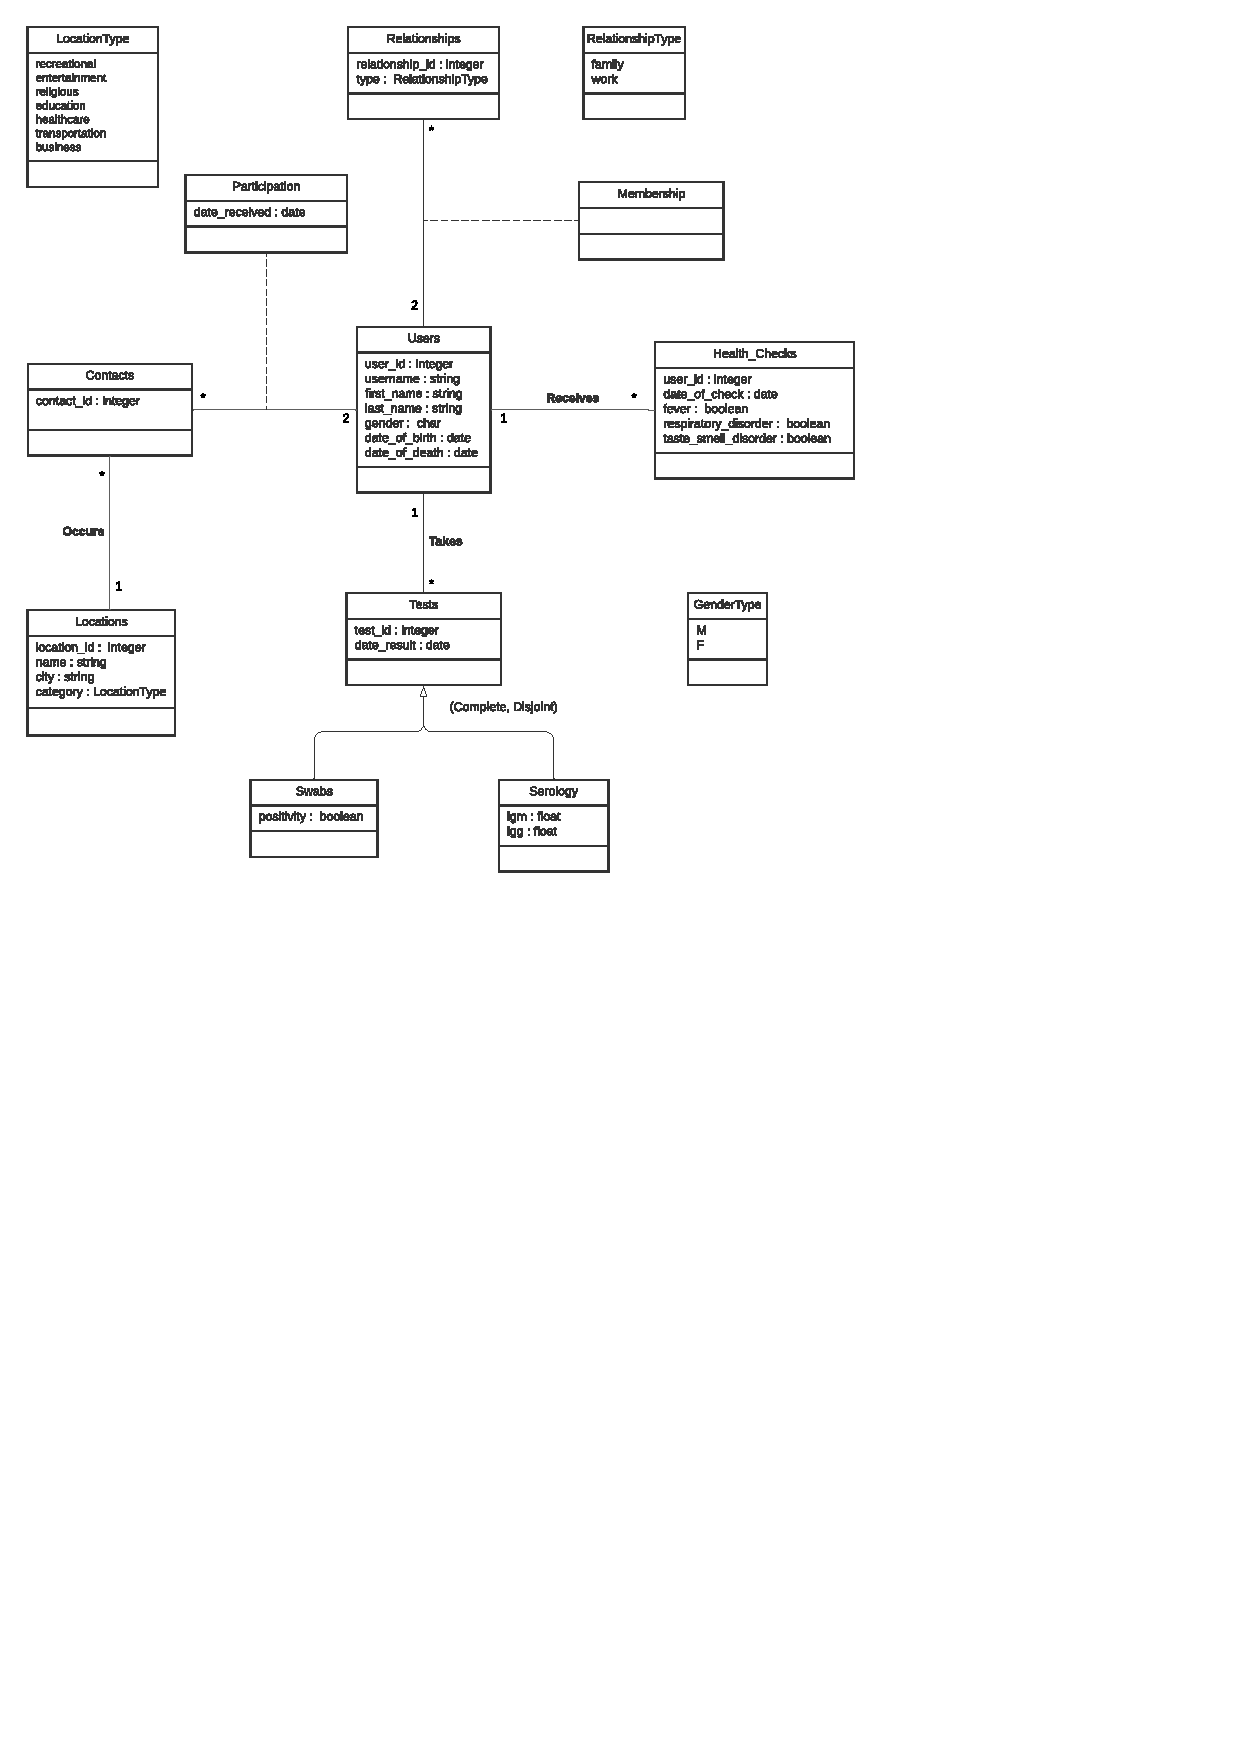
\includegraphics{ClassDiagram.pdf}
    
    \section{Ristrutturazione del class diagram}
    	Affinchè il class diagram sia idoneo alla traduzione in schemi relazionali si deve procedere alla sua ristrutturazione, ovvero eliminare attributi strutturati, attributi multipli, generalizzazioni e specializzazioni.
    	
    	\subsection{Rimozione delle specializzazioni}
    		La specializzazione di \textbf{Tests} in \textbf{Swabs} e \textbf{Serological tests}, essendo di tipo totale e disgiunta, verrà eliminata "schiacciando" la superclasse nelle sottolassi.
    		
    		%\includegraphics{imagefile}
    	
    \subsection{Valutazione ulteriore}
    	Procedendo con la costruzione del database ci siamo resi conto delle varie problematiche che sorgevano a causa di associazioni simmetriche e per ovviare a questo problema abbiamo strutturato il tutto in modo che sia più efficiente sia in termini di spazio che di velocità di ricerca, il risultato finale è il seguente:
    	
    	%\includegraphics{imagefile}
    	    	
    	\section{Dizionario dei dati}
    
    		\subsection{Dizionario delle classi}
    		
    		\begin{tabularx}{\textwidth}{lXX}
    		\toprule
    		Classe & Descrizione & Attributi \\
    		\midrule
    		\multirow{6}*{\textbf{User}} & Descrittore di ciascun utente presente nella collezione di dati. & \textbf{User\_id} (string): chiave sintetica per identificare univocamente un user.\\&& 
    		\textbf{Username} (string): \\&&
    		\textbf{First\_Name} (string): Nome dell'utente.\\&&
    		\textbf{Last\_name} (string): Cognome dell'utente.\\&&
    		\textbf{Gender} (char): sesso dell'utente.\\&&
    		\textbf{Date\_of\_birth} (date): data di nascita dell'utente.\\&&
    		\textbf{Date\_of\_death} (date): possibile data di morte dell'utente.\\
    		\midrule
    		
    		\multirow{3}* {\textbf{Swab}} & Descrittore di ogni possibile tampone a cui un utente si è sottoposto. & 
    		\textbf{Swab\_id} (integer): chiave sintetica per identificare univocamente uno swab.\\&&
    		\textbf{Date\_result} (date): data in cui si è ottenuto il risultato del tampone.\\&&
    		\textbf{Positivity} (char): eventuale positività o negatività del tampone.\\
    		\midrule
    		
    		\multirow{4}* {\textbf{Serological\_test}} & Descrittore di ogni possibile test seriologico a cui un utente si è sottoposto. & 
    		\textbf{Serological\_test\_id} (integer): chiave sintetica per identificare univocamente un test sierologico.\\&&
    		\textbf{Date\_result} (date): data in cui si è ottenuto il risultato del test.\\&&
    		\textbf{IGM} (char): eventuale presenza di anticorpi IGM.\\&&
    		\textbf{IGG} (char): eventuale presenza di anticorpi IGG.\\
    		\midrule
    		
    		\multirow{5}* {\textbf{Health\_check}} & Descrittore del quadro clinico di ogni utente per data di controllo. & 
    		\textbf{Health\_check\_id} (integer): chiave sintetica per identificare univocamente ogni quadro clinico di un utente.\\&&
    		\textbf{Date\_of\_check} (date): data in cui è avvenuto il controllo sullo stato di salute dell'utente.\\&&
    		\textbf{Fever} (char): eventuale presenza del sintomo della febbre.\\&&
    		\textbf{Respiratory\_disorder} (char): eventuale presenza del sintomo della mancanza di fiato.\\&&
    		\textbf{Smell\_taste\_disorder} (char): eventuale presenza del sintomo della perdità del senso del gusto e dell'olfatto.\\
    		\midrule
    		
    		\multirow{2}* {\textbf{Membership}} & Descrittore dell'appartenenza ad una relazione. & 
    		\textbf{User\_id} (integer): chiave esterna per identificare a quale user ci si riferisce.\\&&
    		\textbf{Relationship\_id} (integer): chiave esterna per identificare a quale relationship ci si riferisce.\\
    		\midrule
    		
    		\multirow{2}* {\textbf{Participant}} & Descrittore dell'appartenenza ad un contatto. & 
    		\textbf{User\_id} (integer): chiave esterna per identificare a quale user ci si riferisce.\\&&
    		\textbf{Contact\_id} (integer): chiave esterna per identificare a quale contact ci si riferisce.\\
    		\midrule
    		
    		\multirow{2}* {\textbf{Relationship}} & Descrittore di una relazione fra due user. & 
    		\textbf{Relationship\_id} (integer): chiave sintetica per identificare univocamente la relazione.\\&&
    		\textbf{type} (string): descrittore del tipo di relazione tra utenti.\\
    		\midrule
    		
    		\multirow{2}* {\textbf{Membership}} & Descrittore dell'appartenenza ad una relazione. & 
    		\textbf{User\_id} (integer): chiave esterna per identificare a quale user ci si riferisce.\\&&
    		\textbf{Relationship\_id} (integer): chiave esterna per identificare a quale relationship ci si riferisce.\\
    		\midrule
    		
    		\multirow{2}* {\textbf{Contact}} & Descrittore dell'appartenenza ad una relazione. & 
    		\textbf{Contact\_id} (integer): chiave sintetica per identificare univocamente ogni contatto.\\&&
    		\textbf{Location\_id} (integer): chiave esterna per identificare a quale location ci si riferisce.\\
    		\midrule
    		
    		\multirow{4}* {\textbf{Location}} & Descrittore dell'appartenenza ad una relazione. & 
    		\textbf{Location\_id} (integer): chiave sintetica per identificare univocamente ogni location.\\&&
    		\textbf{Name} (string): Descrittore del nome del luogo.\\ &&
    		\textbf{City} (string): Descrittore della città in cui è presente il luogo.\\ &&
    		\textbf{Category} (string): Descrittore del tipo di luogo.\\ 
    		
    		\bottomrule
    	\end{tabularx}
    
    		\subsection{Dizionario delle associazioni}
    	
    		
    		\begin{tabularx}{\textwidth}{lXX}
    			\toprule
    			Nome & Descrizione & Classi Coinvolte \\
    			\midrule
    			\multirow{2}*{\textbf{Takes}} & Esprime l'aver fatto un tampone o un test seriologico.&
    			\textbf{User [1]} : indica l'utente che ha effettuato uno dei due test\\&&
    			\textbf{Swab (Serological\_test)[*]} : indica i test effettuati dagli utenti.\\
    			\midrule
    			
    			\multirow{2}*{\textbf{Receives}} & Esprime l'aver ricevuto un quadro clinico.&
    			\textbf{User [1]} : indica l'utente che ha ricevuto il quadro clinico\\&&
    			\textbf{Healt\_check[*]} : indica i quadri clinici ricevuti dagli utenti.\\
    			\midrule
    			
    			\multirow{2}*{\textbf{Takes}} & Esprime l'aver fatto un tampone o un test seriologico.&
    			\textbf{User [1]} : indica l'utente che ha effettuato uno dei due test\\&&
    			\textbf{Swab (Serological\_test)[*]} : indica i test effettuati dagli utenti.\\
    			\midrule
    			
    			\multirow{2}*{\textbf{Occurs}} & Esprime l'occorenza di un determinato contatto in un determinato luogo.&
    			\textbf{Location [1]} : indica il luogo in cui è avvenuto il contatto\\&&
    			\textbf{Swab (Contact)[*]} : indica i contatti avvenuti.\\
    			\bottomrule
    			
    		\end{tabularx}
	
\chapter{Progettazione logica}
	In questo capitolo sarà trattata la fase successiva della progettazione della base di dati scendendo ad un livello di astrazione più basso rispetto alla precedente. Si tradurrà lo schema concettuale(già predisposto in seguito alla ristrutturazione) in uno schema logico, dipendente dal tipo di struttura dei dati prescelto cioè quello relazionale puro. Negli schemi relazionali che seguiranno le chiavi primarie sono indicate con una singola sottolineatura mentre le chiavi esterne con una doppia sottolineatura.
	
		\section{Traduzione in schemi relazionali}
		
			\textbf{USER}(\underline{\textbf{User\_id}}, Username, First\_name, Last\_name, Gender, Place\_of\_birth, Date\_of\_birth, Date\_of\_death)\\
			\textbf{Chiavi esterne:} nessuna.\\
			
			\textbf{SWAB} (\underline{\textbf{Swab\_id}}, \underline{\underline{\textbf{User\_id}}}, Date\_result, Positivity)\\
			\textbf{Chiavi esterne:} User\_id ----> USER.User\_id.\\
			
			\textbf{SEROLOGICAL\_TEST} (\underline{\textbf{Serological\_test\_id}}, \underline{\underline{\textbf{User\_id}}}, Date\_result, IGM, IGG)\\
			\textbf{Chiavi esterne:} User\_id ----> USER.User\_id.\\
			
			\textbf{HEALTH\_CHECK} (\underline{\textbf{Health\_check\_id}}, \underline{\underline{\textbf{User\_id}}}, Date\_of\_check, Fever, Respiratory\_disorder, Smell\_taste\_disorder)\\
			\textbf{Chiavi esterne:} User\_id ----> USER.User\_id.\\
			
			\textbf{MEMBERSHIP} (\underline{\underline{\textbf{User\_id}}}, \underline{\underline{\textbf{Relationship\_id}}})\\
			\textbf{Chiavi esterne:} User\_id ----> USER.User\_id;\\ Relationship\_id ----> RELATIONSHIP.Relationship\_id.\\
			
			\textbf{PARTICIPANT} (\underline{\underline{\textbf{User\_id}}}, \underline{\underline{\textbf{Contact\_id}}})\\
			\textbf{Chiavi esterne:} User\_id ----> USER.User\_id;\\
			Contact\_id ----> CONTACT.Contact.Contact\_id.\\
			
			\textbf{RELATIONSHIP} (\underline{\textbf{Relationship\_id}}, Type)\\
			\textbf{Chiavi esterne:} nessuna.\\
			
			\textbf{CONTACT} (\underline{\textbf{Contact\_id}}, \underline{\underline{\textbf{Location\_id}}})\\
			\textbf{Chiavi esterne:} Location\_id ----> LOCATION.Location\_id.\\

\end{document}
